%% abtex2-modelo-livro.tex, v-1.9.6 ycherem
%% Copyright 2012-2016 by abnTeX2 group at http://www.abntex.net.br/
%%
%% This work may be distributed and/or modified under the
%% conditions of the LaTeX Project Public License, either version 1.3
%% of this license or (at your option) any later version.
%% The latest version of this license is in
%%   http://www.latex-project.org/lppl.txt
%% and version 1.3 or later is part of all distributions of LaTeX
%% version 2005/12/01 or later.
%%
%% This work has the LPPL maintenance status `maintained'.
%%
%% Further information is available on 
%% http://www.abntex.net.br/
%%
%% This work consists of the files
%% abntex2-modelo-livro.tex, abntex2-modelo-references.bib,   
%% abntex2-modelo-livro-pintassilgo.jpg,
%% abntex2-modelo-livro-saira-amarela.jpg,
%% abntex2-modelo-livro-bandeirinha.jpg
%%

\documentclass[
	% -- opções da classe memoir --
	14pt,				% tamanho da fonte
	openright,			% capítulos começam em pág ímpar (insere página vazia caso preciso)
	oneside
%	twoside,			% para impressão em recto e verso. Oposto a oneside
	a4paper,			% tamanho do papel. 
	% -- opções da classe abntex		2 --
	chapter=TITLE,		% títulos de capítulos convertidos em letras maiúsculas
	section=TITLE,		% títulos de seções convertidos em letras maiúsculas
	subsection=TITLE,	% títulos de subseções convertidos em letras maiúsculas
	subsubsection=TITLE,% títulos de subsubseções convertidos em letras maiúsculas
	% -- opções do pacote babel --
	english,			% idioma adicional para hifenização
	french,				% idioma adicional para hifenização
	spanish,			% idioma adicional para hifenização
	brazil,				% o último idioma é o principal do documento
	sumario=tradicional
]{abntex2}

\usepackage{microtype} 				% para melhorias de justificação
\usepackage[dvipsnames]{xcolor} 	% para cores
\usepackage{graphicx} 				% para imagens
\usepackage{booktabs,tabularx,rotating}% para tabelas
\usepackage{mdframed} 				% para caixas de texto como na CIP do verso do título
\usepackage{multicol}				% tabelas com colunas mescladas
\usepackage{lettrine}				% letras capitulares
\usepackage{xspace} 				% para nao precisar de espaços com {} depois de comandos
									% como \LaTeX e abreviações criadas pelo usuário
\usepackage{lipsum} 				% para texto de preenchimento de exemplo
\usepackage{leading}				% espaçamento entrelinhas (leading)
\leading{13pt}


% ---
% Pacotes de citações
% ---
\usepackage[brazilian,hyperpageref]{backref}	 % Paginas com as citações na bibl
\usepackage[num]{abntex2cite}	% Citações padrão ABNT

% ---
% Configurações do pacote backref
% Usado sem a opção hyperpageref de backref
\renewcommand{\backrefpagesname}{Citado na(s) página(s):~}
% Texto padrão antes do número das páginas
\renewcommand{\backref}{}
% Define os textos da citação
\renewcommand*{\backrefalt}[4]{
	\ifcase #1 %
		Nenhuma citação no texto.%
	\or
		Citado na página #2.%
	\else
		Citado #1 vezes nas páginas #2.%
	\fi}%
% ---

% ---
% Informações do documento
% ---
\titulo{Manual do Usuário - v1}
%\\\textcolor{red}{\textcopyright COPYRIGHT CAMPOS, A.V.G.}}
\autor{Antonio V. G. Campos}
\data{\today}
\preambulo{Copyright \imprimirautor \space \& \imprimirinstituicao \space \textcopyright \space 2021}
\local{São Luis}
\instituicao{3D EasyCAE}


% alterando o aspecto das cores do texto
\usepackage{xcolor}
\definecolor{cinza3deasycae}{RGB}{128, 128, 128}
\definecolor{azul3deasycae}{RGB}{102, 153, 255}
\definecolor{verde3deasycae}{RGB}{0, 204, 102}
\definecolor{laranja3deasycae}{RGB}{255, 102, 102}
\definecolor{laranja33deasycae}{RGB}{255, 204, 153}
\definecolor{amarelo3deasycae}{RGB}{255, 204, 0}


% informações do PDF
\makeatletter
\hypersetup{
     	%pagebackref=true,
		pdftitle={\@title}, 
		pdfauthor={\@author},
    	pdfsubject={\imprimirpreambulo},
	    pdfcreator={LaTeX with abnTeX2},
		pdfkeywords={abnt}{latex}{abntex}{abntex2}{livro}, 
		colorlinks=true,       		% false: boxed links; true: colored links
    	linkcolor=azul3deasycae,          	% color of internal links
    	citecolor=laranja3deasycae,        		% color of links to bibliography
    	filecolor=amarelo3deasycae,      		% color of file links
		urlcolor=verde3deasycae,
%		bookmarksdepth=4
}
\makeatother
% ---


% ---
% Estilo de capítulos
%
% \chapterstyle{pedersen} 
% \chapterstyle{lyhne} 
\chapterstyle{madsen}
%\chapterstyle{veelo} 
%
% Veja outros estilos em:
% https://www.ctan.org/tex-archive/info/MemoirChapStyles
% ---

% para cabeçalhos sem estar em maiúsculas
%\nouppercaseheads
% -----
% Declarações de cabecalhos 
% -----
% Cabecalho padrao
\makepagestyle{abntbookheadings}
\makeevenhead{abntbookheadings}{\ABNTEXfontereduzida\thepage}{}{\ABNTEXfontereduzida\textit\leftmark}
\makeoddhead{abntbookheadings}{\ABNTEXfontereduzida\textit\rightmark}{}{\ABNTEXfontereduzida\thepage}
\makeheadrule{abntbookheadings}{\textwidth}{\normalrulethickness}

% Cabecalho do inicio do capitulo
\makepagestyle{abntbookchapfirst}
\makeoddhead{abntbookchapfirst}{}{}{}

% Configura layout para elementos textuais
\renewcommand{\textual}{%
  \pagestyle{abntbookheadings}%
  \aliaspagestyle{chapter}{abntbookchapfirst}% customizing chapter pagestyle
  \nouppercaseheads%
  \bookmarksetup{startatroot}% 
}
% ---

% ---
% Espaçamentos entre linhas e parágrafos
% ---
% O tamanho do parágrafo é dado por (exemplo):
\setlength{\parindent}{1.3cm}
%% Não recomendado mudar.
 
% Controle do espaçamento entre um parágrafo e outro:
\setlength{\parskip}{0.2cm}  % tente também \onelineskip
%% Não recomendado mudar.

% Margens do documento 
%% (margens do abntex2 não combinam nem com A5 nem com estilos de capítulo da
% classe memoir.)
\setlrmarginsandblock{2.5cm}{3.5cm}{*}
\setulmarginsandblock{2.5cm}{3.5cm}{*}
\checkandfixthelayout
% ---

% Pacotes Não nativos
\usepackage{bm}
\usepackage{emptypage}			 		% Retira o número de páginas em branco
\usepackage{indentfirst}                % Identação do primeiro parágrafo
\usepackage{fancyhdr}                   % Controlar os cabeçalhos e rodapés
\usepackage{amsmath}
\usepackage{amsfonts}
\usepackage{amssymb}
\usepackage{subfig}
\usepackage{float}
\usepackage{hyperref}
\usepackage{floatflt}                   % Quebra de texto em figuras e tabelas
\usepackage{colortbl}                   % Adicionar cor às tabelas
\usepackage{fancyvrb}                   % Texto verbatim sofisticado
\usepackage{wrapfig}                    % Produz figuras que o texto pode ficar ao redor
\usepackage{multirow}
\usepackage{textcomp}
\usepackage{emptypage}
\usepackage{amsmath,amsfonts,amssymb,amsthm,epsfig,epstopdf,titling,url,array}
\usepackage{parskip}
\usepackage[final]{pdfpages}
\usepackage{psfrag}
\usepackage{cancel} % cancelar termos matematicos
\usepackage{tikz}
\usetikzlibrary{backgrounds}
\usetikzlibrary{positioning}

% Pacotes para inserir códigos fontes
% Configurando layout para mostrar codigos
\usepackage{listings}

\lstset{
	language=Python,
	basicstyle=\ttfamily\small,
	keywordstyle=\color{laranja3deasycae},
	stringstyle=\color{verde3deasycae},
	commentstyle=\color{azul3deasycae},
	backgroundcolor=\color{laranja33deasycae},
    breakatwhitespace=false,         
	breaklines=true,                 
	captionpos=b,                    
	keepspaces=true,                 
	numbers=left,                    
	numbersep=5pt,                  
	showspaces=false,                
	showstringspaces=false,
	showtabs=false,                  
	tabsize=2,
	xleftmargin=0.1cm,
	frame=lrtb,
%	framesep=0.5cm,
%	framerule=0pt,
}
\pagestyle{empty}


%
%
%%%%% MARCA D'AGUA SELO
\usepackage[printwatermark]{xwatermark}
\newwatermark*[allpages,color=red!100,angle=45,scale=1,xpos=0,ypos=0]{\imprimirpreambulo}


%%%%% creative commons license
\usepackage{fontawesome}
\usepackage[
type={CC},
modifier={by-nc-nd},
version={4.0},
]{doclicense}

% ---
% Início do documento
% ---
\begin{document}
%% ---
%% Capa principal
%% ---
\begin{titlingpage}
\begin{tikzpicture}[overlay,remember picture,nodes={inner sep=0pt,outer sep=0pt}]
	\draw[white,fill=cinza3deasycae] (current page.north west) rectangle
	++(\paperwidth,-3cm) node[midway,font=\bfseries,align=center,scale=2]{\imprimirautor};
	\draw[white,top color=laranja33deasycae, bottom color=laranja3deasycae] ([yshift=-20cm]current page.north west)
	rectangle   ++(\paperwidth,-6cm)node[midway,font=\bfseries,align=center,scale=1.4]
	{%
	{\large MYFEMPY v9.9.9}\\
	{\Large MANUAL DO USUÁRIO}\\
	{}\\
	{\imprimirdata}\\
	};
\end{tikzpicture}
	
\phantom{xxx}
\vspace{0.5cm}
\huge
\raggedright
\centering 

%\vspace{1.0cm}
\begin{center}
	
\includegraphics[width=1\linewidth]{capa_v1}
\end{center}

% ---
% Verso da contra-capa
% ---
\clearpage
\ABNTEXfontereduzida
\imprimirpreambulo\\
\vspace{1.0cm}
\raggedright
{\large \textbf{DIREITOS AUTORAIS E DISTRIBUIÇÃO}}\\
\vspace{0.5cm}
O autor é o principal responsável por todas as informações contidas aqui apresentadas, podendo ser utilizadas para qualquer fins legais, desde que devidamente citado. Entretanto, não há garantias explicitas de que o uso de tais informações produza sempre o resultado desejado.\\
\vspace{0.5cm}

\textbf{Todos os direitos reservados}. Esta obra possui direitos autorais vinculados, qualquer reprodução de partes desta publicação é estreitamente proibida e passível de punição por lei.\\
\vspace{0.5cm}

A distribuição legal desta obra é de direitos da 3D EasyCAE.

\begin{center}
	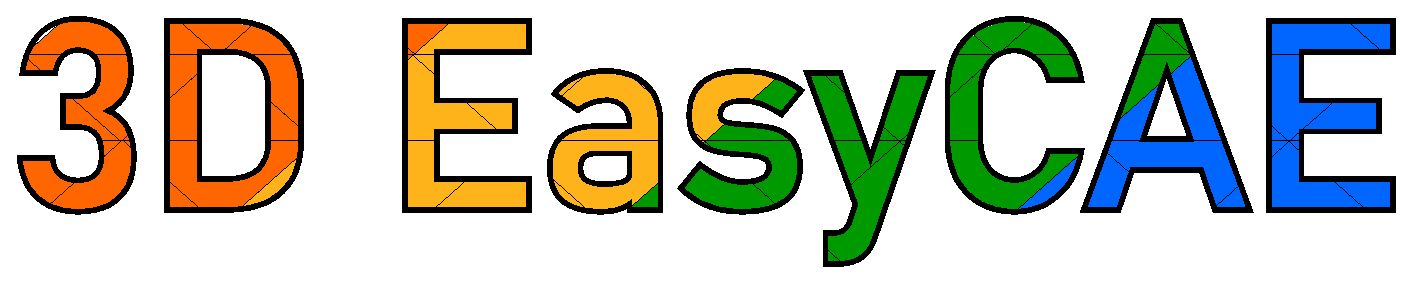
\includegraphics[width=0.7\linewidth]{logoNome2_svg}
\end{center}
%\raggedright
$ $\\
Para dúvidas e sugestões entre em contato pelo e-mail \textbf{elementosfinitos.querosaber@gmail.com}.

\vspace*{\fill}
Todas as figuras, imagens e ilustrações autorais contidas nesta obra estão sob a licença \doclicenseName.\\
\begin{center}
	\doclicenseImage
\end{center}
Todas as figuras, imagens e ilustrações de terceiros possuem licença livre própria devidamente citada.\\
%\doclicenseThis
\end{titlingpage}

\begin{agradecimentos}
%\medskip
\end{agradecimentos}
% ---
% ---
% inserir o sumario
% ---
\pdfbookmark[0]{\contentsname}{toc}
\tableofcontents* 
\cleardoublepage
% ---
% ------------------------------------------------------------
% Início da parte textual
% ------------------------------------------------------------
%\textual
\mainmatter
% ------------------------------------------------------------
%\include{NOTA}
\newpage
%\part{Tópicos em Mecânica Clássica de Estruturas}
%\include{INTROD_MECSOL}
%\include{ESFORC_INTERN}
%\include{TENSAO_DEFORM}
%\include{TENSAO_ESTRUT}
%\include{MODELO_ESTRUT}
%\include{CRITER_FALHAS}
%%%% 
%\part{Introdução à Dinâmica de Estruturas}
%\include{DINAMI_LUMPED}
%\include{DINAMI_VALIDA}
%\include{DINAMI_CONTIN}
%%
%\part{Análise Numérica de Estruturas}
%\include{ELEFIN_BASICO}
%\include{ELEFIN_AVANCA}



% ------------------------------------------------------------
\postextual % pós-textual
% ------------------------------------------------------------
% ------------------------------------------------------------
%------------------------------------------------------------------%
% referencias
%\bibliographystyle{abnt-num}
\bibliography{Mechanical_Solids_Mybook}
% ------------------------------------------------------------
\newpage
\begin{tikzpicture}[overlay,remember picture,nodes={inner sep=0pt,outer sep=0pt}]
	\draw[white,fill=cinza3deasycae] (current page.north west) rectangle
	++(\paperwidth,-3cm) node[midway,font=\bfseries,align=center,scale=2]{};
		
	\draw[white,top color=laranja33deasycae, bottom color=laranja3deasycae] ([yshift=-20cm]current page.north west)
	rectangle   ++(\paperwidth,-6cm)node[midway,font=\bfseries,align=center,scale=1.5]
	{};
\end{tikzpicture}

\begin{center}
	BACK COVER
\end{center}

\end{document}